\documentclass[magisterska]{pracamgr}

\usepackage{polski}
\usepackage[noend]{algpseudocode}
\usepackage[utf8]{inputenc}
\usepackage{graphicx}
%\usepackage{float}
\usepackage{wrapfig}
\usepackage{hyperref}
\usepackage{placeins}
\usepackage{amsfonts}
\usepackage{amssymb}
\usepackage{amsmath}
\usepackage{setspace}

\singlespacing

\newtheorem{theorem}{Twierdzenie}[chapter]
\newtheorem{lemma}[theorem]{Lemat}
\newtheorem{proposition}[theorem]{Stwierdzenie}
\newtheorem{corollary}[theorem]{Wniosek}
\newtheorem{definition}[theorem]{Definicja}


\newenvironment{proof}[1][Dowód]{\begin{trivlist}
\item[\hskip \labelsep {\bfseries #1}]}{\end{trivlist}}
\newenvironment{example}[1][Przykład]{\begin{trivlist}
\item[\hskip \labelsep {\bfseries #1}]}{\end{trivlist}}
\newenvironment{remark}[1][Uwaga]{\begin{trivlist}
\item[\hskip \labelsep {\bfseries #1}]}{\end{trivlist}}

\allowdisplaybreaks


%\floatstyle{boxed}
%\restylefloat{figure}
%\floatplacement{figure}{H}

\author{Jakub Tlałka}
\nralbumu{292665}

\title{Heurystyczna modyfikacja techniki CFR w Pokerze}
\tytulang{Heuristic modification of CFR technique in Poker}

\kierunek{Informatyka}

\opiekun{dra Jakuba Pawlewicza\\
  Wydzia{\l} Matematyki Informatyki i Mechaniki\\
  }
  
\date{Sierpień 2014}

\dziedzina{
11.4 Sztuczna Inteligencja\\
}

\klasyfikacja{
I. Computing Methodologies \\
I.2 ARTIFICIAL INTELLIGENCE \\
I.2.8 Problem Solving, Control Methods, and Search \\
}

\keywords{poker, Texas Holdem, bot, równowaga Nasha, CFR}
 
\newtheorem{defi}{Definicja}[section]

\begin{document}
\maketitle

\begin{abstract}
Tematem pracy jest zbadanie modyfikacji metody CFR. Metoda CFR znajduje
duże zastosowanie w dziedzinie sztucznej inteligencji. Jest wykorzystywana między innymi
w tworzeniu inteligentnych programów do gry Texas Holdem Poker. Modyfikacja
tej metody, opisana w pracy, może pozwolić na tworzenie lepszych strategii niż przy wykorzystaniu
zwykłej wersji CFR.
\end{abstract}

\tableofcontents

\chapter{Wstęp}

\noindent
Ludzie grają w gry już od kilku tysięcy lat. Od zawsze były formą rozrywki oraz integracji.
Zarówno gry sportowe jak i umysłowe stwarzają okazje do rywalizacji, która ma charakter pozytywny, ponieważ
stymuluje do rozwoju nie tylko jednostki, ale i całe społeczności. Rozwój gier komputerowych był równoległy
z rozwojem sprzętu komputerowego. Gry znalazły zastosowanie również w naukach
ekonomicznych. Rozwój teorii gier pomógł zrozumieć procesy rządzące rywalizacją w szeroko rozumianym
znaczeniu. Zdefiniowanie pojęcia równowagi przez amerykańskiego matematyka Johna Nasha \cite{nash} było przełomowym
osiągnięciem w dziedzinie badań nad strategiami, nie tylko w grach, ale i w ekonomii. \\

\noindent
Wraz z rozwojem technologii komputerowych, uzyskano dostęp do narzędzi pozwalających na zastosowanie
teorii do obliczania optymalnych strategii w grach. Powszechnie znana jest rywalizacja
arcymistrzów szachowych z komputerowymi programami. W 1997 roku maszyna "Deep Blue", opracowana przez IBM
specjalnie do celów rywalizacji szachowej, pokonała arcymistrza Garry'ego Kasparova \cite{kasparov}. W przypadku gier
o niewielkim zbiorze stanów, komputery są zdolne obliczyć strategię optymalną, czyli taką, która
gwarantuje najlepszy możliwy dla gracza wynik. Przykładem takiej gry są warcaby. W 2007 roku udowodniono, że programu warcabowego
"Chinook" nie da się pokonać. \cite{chinook} \\

\noindent
Wciąż pozostało jednak wiele gier o rozmiarze tak dużym, że znalezienie dla nich optymalnej strategii wydaje
się poza zasięgiem współczesnych maszyn. Są natomiast bardzo udane próby znajdowania strategii aproksymacyjnych,
liczonych dla abstrakcji rzeczywistych gier, które spisują się coraz lepiej w pojedynkach z ludźmi.
Abstrakcje zawężają zbiór akcji dostępnych graczom i utożsamiają niektóre stany gry w celu zmniejszenia jej rozmiaru.
W trakcie badań nad strategiami rozwinęły się algorytmy takie jak "Monte Carlo Tree Search" \cite{monte-carlo-survey}, czy opisywana
w tej pracy metoda "Counterfactual Regret Minimization" (CFR). Odkrycie tej ostatniej w 2007 roku \cite{cfr} było przełomem
w znajdowaniu aproksymacji równowagi Nasha w grach w postaci ekstensywnej. Metoda modyfikuje strategię w kolejnych iteracjach.
Prawdopodobieństwo zagrania akcji w następnej iteracji jest proporcjonalne do oczekiwanego zysku z tej akcji
przy założeniu, że gracze grają strategią z obecnej iteracji. Końcowa strategia jest strategią uśrednioną ze wszystkich iteracji.
Modyfikacje metody CFR są używane do znajdowania najlepszych istniejących strategii między innymi w grze Texas Holdem Poker. \\

\noindent
Celem tej pracy jest zbadanie algorytmu DAG CFR - modyfikacji algorytmu CFR, która pozwala na wyliczanie strategii w bardziej wiernej
abstrakcji gry Texas Holdem Poker. Odbywa się to kosztem założenia o pełnej pamięci gry (\emph{perfect recall}).
Zignorowanie historii dotychczasowej rozgrywki przy obliczaniu strategii, pozwala na znaczące zmniejszenie liczby
stanów gry przeglądanych w każdej iteracji algorytmu. Pozwala to zmniejszyć liczbę ograniczeń nakładanych
na oryginalną wersję Texas Holdem Poker. Praca bada, czy tak zmodyfikowany algorytm pozwala na znalezienie
lepszych strategii niż oryginalna wersja CFR. \\

\noindent
Rozdział 2 opisuje podstawowe pojęcia i zagadnienia sztucznej inteligencji w grach, takie jak
stan gry, zbiór informacyjny, drzewo gry, strategia. W dalszej części opisane są zasady gry
Texas Holdem Poker, którą wykorzystano do porównania skuteczności metody CFR i jej modyfikacji - DAG CFR.
Zostanie też przybliżona historia rozwoju programów grających w gry oraz metody budowania abstrakcji gier. \\

\noindent
Rozdział 3 opisuje algorytm CFR, w wersji pierwszy raz przedstawionej w 2007 roku w pracy \cite{cfr}.
Zostały w nim przytoczone pojęcia
związane z grami ekstensywnymi oraz twierdzenia dowodzące skuteczności metody CFR. Na końcu rozdziału
zamieszczony jest pseudokod algorytmu $\Call{VanillaCfr}{}$, który jest jednym ze znanych sposobów realizacji metody CFR. \\

\noindent
Rozdział 4 jest poświęcony algorytmowi DAG CFR. Na początku przedstawiona jest idea algorytmu.
Dalej opisana jest wersja gry Texas Holdem Poker zastosowana w eksperymentach. Godny uwagi
jest opisany w tej części pomysł na bardziej efektywne obliczanie metryki $EHS$ dla układów kart.
Wartość $EHS$ wyznacza siłę układu kart. Dzięki jej obliczeniu, możliwe jest utożsamianie układów
o podobnej sile. Jest to stosowane w celu zmniejszenia rozmiaru gry, dla której liczona jest strategia.
Zbiór utożsamionych ze sobą układów o podobnej sile nazywamy koszykiem.
Główna część rozdziału jest poświęcona efektywnej realizacji pomysłu na zmniejszenie złożoności
metody CFR. Opisane są modyfikacje algorytmu $\Call{VanillaCfr}{}$, które pozwalają zmniejszyć złożoność
jego iteracji do liniowej względem liczby różnych stanów, zamiast liniowej względem rozmiaru drzewa gry.
Na końcu zamieszczony został pseudokod algorytmu DAG CFR. \\

\noindent
Rozdział 5 przedstawia wyniki eksperymentalne. Porównane są w nim strategie wyliczone metodą
CFR oraz DAG CFR, przy zastosowaniu kilku wariantów gry. Warianty różnią się pod względem
liczby koszyków, do których przydzielane są układy kart. Podstawowym kryterium
do porównywania jest wynik rzeczywistej rozgrywki Pokera między dwoma programami. Okazuje się,
że metoda DAG CFR pozwala uzyskiwać lepsze strategie nawet przy krótszym czasie obliczeń. \\

\noindent
Rozdział 6 przedstawia podsumowanie wyników pracy. Opisane są zalety badanego podejścia
i możliwości jego poprawy w celu uzyskania jeszcze lepszych strategii.

\chapter{Wprowadzenie do Pokera}

\noindent
W tym rozdziale przybliżona została dziedzina sztucznej inteligencji w grach. Przedstawione
są podstawowe pojęcia i metody. Opisana została gra Texas Holdem Poker, która jest
wykorzystywana do badania algorytmów w tej pracy. Przybliżona została też idea
zmniejszania rozmiaru gry na potrzeby efektywnego obliczania strategii.

\section{Pomocnicze pojęcia}

\begin{definition}
      \textbf{Stan gry} jest rezultatem dotychczasowych akcji podjętych przez graczy oraz zdarzeń losowych.
      Składają się na niego informacje, które opisują aktualną rozgrywkę.
      Stan gry jednoznacznie definiuje zbiór dostępnych
      akcji oraz gracza, który je wykonuje (wliczając w to gracza losowego, który odpowiada
      za generowanie zdarzeń losowych zgodnie z zasadami gry). Wykonywane przez gracza akcje
      zmieniają stan gry (inaczej ich wykonywanie nie ma sensu).
\end{definition}

\begin{definition}
      \textbf{Graf gry} to graf skierowany, którego wierzchołkami są stany gry. Krawędź prowadzi od stanu
      $s_1$ do stanu $s_2$, jeśli w stanie $s_1$ można wykonać akcję prowadzącą do stanu
      $s_2$. Jeśli w takim grafie nie występuje cykl, nazywamy go DAGiem.
\end{definition}

\begin{definition}
      \textbf{Drzewo gry} reprezentuje wszystkie możliwe rozgrywki. Każdy wierzchołek reprezentuje jedną historię,
      czyli ciąg akcji wykonanych w grze. Wierzchołkowi przypisany jest stan gry, który jest efektem
      wykonania tego ciągu akcji. Z każdego wierzchołka wychodzi tyle krawędzi, ile różnych
      akcji można wykonać w stanie gry przypisanym temu wierzchołkowi.
\end{definition}

\begin{definition}
      Gry dzielimy na dwie kategorie: \textbf{z pełną informacją} oraz \textbf{z niepełną informacją}.
      W przypadku tych pierwszych, wszyscy gracze posiadają wszystkie informacje o zdarzeniach
      zachodzących w grze. Przykładem takiej gry są szachy. W grach z niepełną informacją niektóre
      zdarzenia są ukryte dla pewnego zbioru graczy. Na przykład w więkości gier karcianych gracze
      nie znają kart swoich przeciwników.
\end{definition}

\begin{definition}
      \textbf{Zbiór informacyjny} dla gracza $p$ zawiera te stany gry, które są identyczne jeśli chodzi
      o informacje dostępne graczowi $p$. Przykładowo, w dwuosobowej grze karcianej przykładem zbioru informacyjnego
      jest zbiór wszystkich stanów zaraz po rozdaniu kart, w których gracz $p$ ma na ręku jedynie asa i króla kier.
      Zbiory informacyjne są ważne z punktu widzenia podejmowania decyzji: w każdym stanie gry należącym do tego
      samego zbioru informacyjnego gracza $p$, gracz $p$ podejmuje decyzje według tej samej strategii.
\end{definition}

\begin{definition}
      \textbf{Strategia} gracza $p$ wyznacza zasady podejmowania przez gracza akcji w zbiorach informacyjnych.
      Strategia może być deterministyczna, jeśli w każdym zbiorze informacyjnym jest wyznaczona dokładnie
      jedna podejmowana akcja, bądź mieszana, jeśli na akcjach określony jest rozkład prawdopodobieństwa
      zagrania ich.
\end{definition}

\begin{definition}
      \textbf{Botem} nazywamy program, który podejmuje akcje w grze zgodnie z zaprogramowaną bądź wyliczoną strategią.
\end{definition}

\section{Sztuczna inteligencja w grach}

Sztuczna inteligencja w grach to dział algorytmiki zajmujący się badaniem programów grających
z dużą skutecznością w gry. Jest dużo rodzajów gier. Gry jednoosobowe to tak zwane łamigłówki, w których
należy znaleźć odpowiednią sekwencję ruchów, prowadzącą do jak najlepszego wyniku. Algorytmy znajdujące
takie sekwencje opierają się na efektywnym przeglądaniu drzewa gry. Programy grające w gry wieloosobowe
muszą wyliczyć odpowiednią strategię. Gry różnią się złożonością informacji składających się na stan gry.
Nawet prosta gra, w której graczom przydzielana jest losowo wybrana liczba rzeczywista, mają nieskończenie
wiele stanów gry. Zazwyczaj jednak informacje można reprezentować przez ograniczone liczby całkowite, przez co
liczba stanów gry też jest ograniczona. Przedmiotem badań tej pracy jest gra Texas Holdem Poker, która
należy do gatunku gier z niepełną informacją, z ograniczoną liczbą stanów gry.

\section{Texas Holdem Poker}

Texas Holdem Poker to gra karciana przeznaczona dla co najmniej dwóch graczy. Na początku pojedynczej rozgrywki każdy z graczy
dostaje dokładnie dwie karty, których nie pokazuje przeciwnikom. Następuje potem runda licytacji, w której
gracze ustalają wysokość stawki. W pierwszej rundzie licytacji gracz zaczynający musi wejść do gry
za stawkę ustaloną wielkością "small blind" a następny gracz w kolejności musi wejść stawką o wysokości
"big blind". \\

\noindent
W licytacji gracze odzywają się w ustalonej kolejności. Mogą wejść za całą dostępną im kwotę (\textbf{all-in}),
podbić stawkę (\textbf{raise}), pozostać przy
obecnej stawce (\textbf{call}) lub zrezygnować z udziału w licytacji (\textbf{fold}). Jeśli nie zrezygnują z licytacji,
są zobowiązani włożyć do puli stawkę, na którą się zgodzili. Różne wersje gry określają ograniczenia podnoszenia
stawki. W tej pracy przyjęta jest wersja, w której można podnieść stawkę o dowolną kwotę całkowitą, o ile stawka
po podniesieniu nie przekracza 128 jednostek. Popularną, ale jednocześnie trudną obliczeniowo wersją,
jest wersja no-limit, w której nie nakłada się limitu na kwotę przebicia.
Stawka na zakończenie licytacji zostaje ustalona, gdy
wszyscy gracze biorący jeszcze udział w licytacji zaakceptują aktualną wysokość stawki. Jeśli będzie to
tylko jedna osoba, zostaje ona zwycięzcą i zgarnia całą pulę a gra się kończy. W limit Texas Holdem Poker
nakłada się ograniczenie na liczbę zagrywek jednego gracza w licytacji.\\

\noindent
Wyróżniamy cztery rundy licytacji.
Po rundzie numer $1$ następuje wyłożenie trzech kart na stół, tak by widzieli je wszyscy gracze.
Na taką trójkę mówi się \emph{flop}. Następuje kolejna runda licytacji, po czym wykładana jest jedna karta, nazywana \emph{turn}.
Po rundzie numer $3$ na stół wykładana jest ostatnia karta - \emph{river} i następuje ostatnia runda
licytacji. Jeżeli w ostatniej rundzie co najmniej dwóch graczy uzgodni ostateczną stawkę gry, następuje
wyłożenie kart graczy na stół i rozstrzygnięcie kto został zwycięzcą. \\

\noindent
Zwycięzcą zostaje gracz, który jest w stanie wybrać ze swoich kart oraz kart na stole, najsilniejszy
5-kartowy układ. Siłę układu 5 kart wyznacza poniższy ranking. Dla każdego typu układu, im wyższe
figury występują w układzie, tym większa jest jego siła. Typy układów wymienione są w kolejności
od najsilniejszego do najsłabszego.

\begin{enumerate}
\item \textbf{Poker}: 5 kolejnych kart w tym samym kolorze, np. $(D\clubsuit, W\clubsuit, 10\clubsuit, 9\clubsuit, 8\clubsuit)$. 
\item \textbf{Kareta}: 4 takie same figury, np. $(7\heartsuit, 7\spadesuit, 7\diamondsuit, 7\clubsuit, D\diamondsuit)$.
\item \textbf{Full}: Trójka takich samych figur oraz para w innej figurze, np. $(K\heartsuit, K\diamondsuit, K\clubsuit, 3\heartsuit, 3\diamondsuit)$. 
\item \textbf{Kolor}: 5 kart w tym samym kolorze, np. $(K\diamondsuit, W\diamondsuit, 6\diamondsuit, 5\diamondsuit, 2\diamondsuit)$.
\item \textbf{Strit}: 5 kolejnych kart, np. $(10\heartsuit, 9\diamondsuit, 8\heartsuit, 7\clubsuit, 6\spadesuit)$.
\item \textbf{Trójka}: 3 takie same figury, np. $(5\heartsuit, 5\diamondsuit, 5\clubsuit, 8\heartsuit, D\spadesuit)$.
\item \textbf{Dwie pary}: Dwie pary tych samych figur, np. $(A\heartsuit, A\diamondsuit, 8\clubsuit, 8\heartsuit, W\clubsuit)$.
\item \textbf{Para}: Para tych samych figur, np. $(10\clubsuit, 10\spadesuit, A\heartsuit, 9\clubsuit, 2\heartsuit)$.
\item \textbf{Najwyższa karta}: Najwyższa figura, np. $(K\heartsuit, W\diamondsuit, 10\heartsuit, 9\heartsuit, 5\spadesuit)$.
\end{enumerate}

\noindent
W sytuacji gdy gracze mają ten sam typ układu, z tymi samymi figurami, pod uwagę brane są pozostałe karty z układu. Na przykład
układ $(7\heartsuit, 7\diamondsuit, 7\clubsuit, K\heartsuit, W\clubsuit)$ jest silniejszy od układu
$(7\spadesuit, 7\diamondsuit, 7\clubsuit, K\spadesuit, 5\diamondsuit)$. \\

\noindent
Jeśli po uwzględnieniu wszystkich 5 kart układu nadal występuje remis (na przykład gdy najsilniejszy układ stanowią karty na stole),
pula jest dzielona między graczy z najwyższym układem.

\section{Rozwój botów grających w Pokera}

Pierwsze boty opierały swoją strategię na zbiorze zasad wpisanych ręcznie przez pokerowych graczy. Zasady określały
sposób podejmowania decyzji w konkretnych sytuacjach, na przykład "Mając na ręku Asa i Damę, podbijaj stawkę trzykrotnie".
W 2004 roku powstał program WinHoldem, który umożliwiał proste tworzenie botów, grających według pewnego zbioru zasad.
Jednocześnie, w środowiskach akademickich, rozwijały się podejścia oparte na znajdowaniu równowagi Nasha. Owocem tych
badań jest między innymi opisywany w tej pracy algorytm CFR \cite{cfr, cfr2, cfr3}. Takie podejścia przeważają w długiej serii rozgrywek, ale
brakuje im umiejętności wykorzystania słabości w strategiach przeciwnika. Powstały również algorytmy, które w serii
rozgrywek próbują estymować strategię przeciwnika i znajdują najlepszą dla niej kontrstrategię \cite{exploit}.

\section{Zmniejszanie drzewa gry}

Drzewo gry w pokerze jest bardzo duże. W dwuosobowym no-limit Texas Holdem Poker ma wielkość
około $10^{70}$ stanów \cite{monte-carlo}. Dlatego niezbędne jest wprowadzenie abstrakcji gry.
Pierwsze ograniczenie, które zastosowano, dotyczy licytacji. Dostępne są maksymalnie 4 akcje:
\textbf{fold} (rezygnacja z licytacji), \textbf{call} (pozostanie przy obecnej stawce), \textbf{raise} (dwukrotne podbicie stawki) oraz
\textbf{all in} (zalicytowanie maksymalnej stawki - 128). W ten sposób jedyne możliwe wysokości stawek w licytacji to: $1$, $2$,
$4$, $8$, $16$, $32$, $64$ i $128$. \\\\
\noindent
Drugie ograniczenie przyporządkowuje układom kart graczy (karty na ręce wraz z kartami na stole) tak zwane \emph{"koszyki"} \cite[punkt 4.4]{buckets}.
W jednym koszyku są karty o podobnej sile. W każdej rundzie licytacji obowiązuje osobny podział, zmienna
jest też liczba koszyków. Testowano różne liczby koszyków, w zależności od używanego algorytmu. \\\\
\noindent
Do oceny siły układów zastosowano miarę "Effective Hand Strength" (EHS) \cite{ehs}. EHS układu wyliczany
jest z trzech innych miar: "Hand Strength" ($HS$), "Positive Potential" ($Ppot$) oraz "Negative Potential" ($Npot$), według
wzoru:

\begin{align*}
EHS = HS \cdot (1 - Npot) + (1 - HS) \cdot Ppot
\end{align*}

\noindent
$HS$ to w przybliżeniu prawdopodobieństwo, że nasza ręka jest lepsza od ręki przeciwnika. Miary $Ppot$ i $Npot$ oznaczają
prawdopodobieństwo, że nasza ręka stanie się lepsza (odpowiednio gorsza) od ręki przeciwnika, po wyłożeniu kolejnych kart na stół. \\

\begin{example}
$\,$ \\\\
\noindent

\noindent
Ręka ($A\heartsuit$, $A\clubsuit$ ; $A\diamondsuit$, $5\spadesuit$, $2\clubsuit$) (dwie pierwsze karty to karty na ręce) ma wartość $HS$
bliską $1$, gdyż żadna możliwa para kart nie tworzy lepszego układu, gdy na stole są karty ($A\diamondsuit$, $5\spadesuit$, $2\clubsuit$). \\

\noindent
Ręka ($3\heartsuit$, $4\clubsuit$ ; $A\diamondsuit$, $5\spadesuit$, $2\clubsuit$) ma wysoką wartość $Ppot$ ponieważ ma niską wartość $HS$,
ale jednocześnie duży potencjał na stanie się ręką z układem \textbf{strit}, gdy dojdą kolejne karty. \\

\noindent
Ręka ($A\heartsuit$, $A\clubsuit$ ; $A\diamondsuit$, $5\diamondsuit$, $2\diamondsuit$) ma wysoką wartość $Npot$ ponieważ jest silna
dzięki parze asów, ale istnieje stosunkowo duże prawdopodobieństwo, że przeciwnik posiada karty w kolorze $\diamondsuit$, co zwiększa jego szansę
na uzyskanie ręki z układem jednokolorowym.

\end{example}


\chapter{Metoda CFR}

Metoda CFR (Counterfactual Regret Minimization) to algorytm, który pozwala znajdować równowagę Nasha
w grach w postaci ekstensywnej. Jest to obecnie najlepsze rozwiązanie w dziedzinie badań nad
sztuczną inteligencją w Pokerze \cite{cfr}. Choć używane są głównie różne modyfikacje algorytmu,
przedstawiona zostanie tu jego bazowa wersja. W punkcie \ref{oznaczenia} przedstawię podstawowe oznaczenia i terminologię
używaną w opisie algorytmu. W punkcie \ref{cfr-opis} zostaną przytoczone definicje i twierdzenia dowodzące skuteczności metody
CFR. Na końcu rozdziału, w punkcie \ref{impl-cfr}, został zamieszczony opis algorytmu $\Call{VanillaCfr}{}$, który liczy strategię zgodnie z metodą CFR.

\section{Oznaczenia}
\label{oznaczenia}

\begin{itemize}

\item Zbiór graczy oznaczamy przez $N$. Graczy numerujemy od $0$, gracza losowego oznaczamy literą $c$.
\item Zbiór wszystkich możliwych ciągów akcji (historii) legalnych w grze nazywamy $H$. Ciągi, po których kończy
      się rozgrywka, należą do podzbioru $Z$. Każdej historii jest przyporządkowany stan gry, który
      jest jej efektem. Historię uzyskaną po wykonaniu akcji $a$ w historii $h$ oznaczamy przez $h \circ a$.
\item Dla każdej historii $h$, zbiór akcji dostępnych w odpowiadajacym jej stanie gry oznaczamy przez $A(h)$.
      Każdy stan wyznacza jednoznacznie gracza wykonującego akcję - $P(h)$.
\item Dla każdego gracza $i$, historie, w których ma on ruch, są pogrupowane w zbiory informacyjne $I_i$. Dla zbioru
      informacyjnego $I_i$ oraz dowolnych dwóch historii $h_1, h_2 \in I_i$, zachodzi $A(h_1) = A(h_2) = A(I_i)$. Do jednego
      zbioru informacyjnego $I_i$ należą historie, które są parami tożsame po usunięciu z nich akcji niewidocznych dla gracza $i$
      (np. w Pokerze są to akcje przydzielenia kart prywatnych graczom innym niż $i$).
\item Funkcja $f_c(h, a)$ oznacza prawdopodobieństwo wykonania przez gracza losowego akcji $a$ przy historii $h$.
\item Strategię gracza $i$ oznaczamy przez $\sigma_i$. $\sigma_i(I_i, a)$ oznacza prawdopodobieństwo wykonania akcji $a$ przez
      gracza $i$ w zbiorze informacyjnym $I_i$, jeśli gra on strategią $\sigma_i$. Przyjmujemy $\sigma_c(h, a) = f_c(h, a)$.
      Przez $\sigma$ oznaczamy zespół strategii wszystkich graczy biorących udział w rozgrywce. Stosujemy też oznaczenie
      zespołu strategii jako $(\sigma_{i_1}, ... \, , \sigma_{i_n})$, czyli zbiór strategii poszczególnych graczy. Przez $\sigma_{-i}$ oznaczamy
      zespół strategii wszystkich graczy z wyjątkiem $i$. $(\sigma'_i, \sigma_{-i})$ oznacza zespół strategii złożony ze strategii
      gracza $i$ wziętej z $\sigma'$ oraz ze strategii pozostałych graczy wziętych z $\sigma$.
\item Przez $\pi^{\sigma}(h)$ oznaczamy prawdopodobieństwo zajścia historii $h$ dla zespołu strategii $\sigma$.
      $\pi^{\sigma}(I)$ to suma tych prawdopodobieństw po $h \in I$. $\pi_i^{\sigma}(h)$ to prawdopodobieństwo że grając
      zgodnie ze strategią $\sigma$, gracz $i$ będzie podejmował akcje z odpowiadającej historii $h$. Analogicznie
      $\pi_{-i}^{\sigma}(h)$ oznacza prawdopodobieństwo że pozostali gracze będą podejmowali akcje z historii $h$. W szczególności
      zachodzi $\pi_{-i}^{\sigma}(h) \, = \, \prod\limits_{i \neq j \in N} \, \pi_j^{\sigma}(h)$.
\end{itemize}

\begin{definition}
      Dla końcowych historii $h \in Z$ określamy \textbf{funkcję użyteczności} $\mu_i(h)$, oznaczającą zysk gracza $i$ w rozgrywce
      określonej przez $h$. Dla historii $h \notin Z$ określamy $\mu_i^{\sigma}(h)$, oznaczającą oczekiwany zysk gracza $i$
      przy założeniu że gracze grają strategią $\sigma$ i historia $h$ została osiągnięta. Funkcja $\mu^{\sigma}$ wyznacza
      oczekiwane zyski graczy w pełnej rozgrywce, przy ustalonym zespole strategii $\sigma$.
\end{definition}

\noindent
W dalszej części będziemy zajmować się grami dwuosobowymi, przede wszystkim dwuosobową wersją Texas Holdem Poker.

\section{$\epsilon$-równowaga Nasha}

\emph{$\epsilon$-równowagą Nasha} nazywamy zespół strategii $\sigma$, taki że:

\begin{align*}
\mu_1^{\sigma} + \epsilon \geq  \max_{\sigma_1'} \, \mu_1^{(\sigma_1', \sigma_2)} 
\end{align*}

\begin{align*}
\mu_2^{\sigma} + \epsilon \geq  \max_{\sigma_2'} \, \mu_2^{(\sigma_1, \sigma_2')} 
\end{align*}

\noindent
Intuicyjnie, strategie graczy są w $\epsilon$-równowadze Nasha, gdy żaden z graczy nie może zmodyfikować swojej strategii
by uzyskać wynik lepszy o więcej niż $\epsilon$ od wyniku jaki uzyskałby grając obecną strategią, przy założeniu, że przeciwnik nie zmienia
swojej strategii.
Metoda CFR znajduje $\epsilon$-równowagę Nasha dla $\epsilon$ malejącego proporcjonalnie do odwrotności pierwiastka z liczby iteracji.

\section{Minimalizacja funkcji regretu}
\label{cfr-opis}

W dalszej części przyjmujemy, że rozgrywane są kolejne rundy indeksowane przez $t$. W każdej z rund
strategie graczy będą modyfikowane na podstawie dotychczasowej rozgrywki, w efekcie dając ciąg strategii
$(\sigma^t)$. Jako \emph{uśrednioną strategię} gracza $i$ po $T$ rundach definiujemy:

\begin{align*}
\overline{\sigma}_i^T(I, a) = \frac{\sum\limits_{t=1}^T \pi_i^{\sigma^t}(I) \, \sigma^t(I, a)}{\sum\limits_{t=1}^T \, \pi_i^{\sigma^t}(I)}
\end{align*}

\noindent
Intuicyjnie, funkcja regretu określa ile gracz mógłby zyskać, zamieniając obecną strategię na najlepszą możliwą,
przy założeniu że inni gracze pozostali by przy obecnych strategiach. Formalnie, definiujemy \emph{średni całkowity regret} gracza $i$
w rozgrywce o numerze $T$ przez:

\begin{align*}
R_i^T = \frac{1}{T} \, \max_{\sigma_i'} \sum\limits_{t=1}^T \, (\mu_i^{(\sigma_i', \sigma_{-i}^t)} - \mu_i^{\sigma^t})
\end{align*}

\noindent
Znany wynik \cite{cfr} mówi o tym, że w grze o sumie zerowej, jeśli po $T$ iteracjach średni całkowity regret obu graczy
jest mniejszy niż $\epsilon$, to uśredniony zespół strategii $\overline{\sigma}^T$ jest $2\epsilon$-równowagą Nasha.

\section{Funkcja regretu lokalnego}

By łatwiej minimalizować regret całkowity, wprowadzamy funkcję regretu lokalnego.
Działa ona na podobnej zasadzie co regret całkowity, ale jest określana na zbiorach informacyjnych
a nie na całej grze. Dzięki temu można ją minimalizować osobno dla każdego zbioru informacyjnego. \\\\

\noindent
Niech $\sigma_{|I \rightarrow a}$ oznacza strategię $\sigma$ zmodyfikowaną tak, że w zbiorze informacyjnym $I$ zawsze
wykonywana jest akcja $a$. $\mu_i(\sigma, I)$ oznacza warunkową wartość oczekiwaną zysku gracza $i$, przy założeniu że
osiągnięty został zbiór informacyjny $I$ a gracze grają strategią $\sigma$, zmodyfikowaną tak, że gracz $i$
podejmuje akcje prowadzące do zbioru informacyjnego $I$ z prawdopodobieństwem $1$. \\\\

\noindent
Wtedy definiujemy \emph{lokalny regret akcji} jako:

\begin{align*}
R_i^T(I, a) = \frac{1}{T} \sum\limits_{t=1}^{T} \, \pi_{-i}^{\sigma^t}(I)(\mu_i(\sigma^t_{|I \rightarrow a}, I) - \mu_i(\sigma^t, I))
\end{align*}

\noindent
oraz \emph{funkcję regretu lokalnego} jako:

\begin{align*}
R_{i, imm}^T(I) = \max_{a \in A(I)} \, R_i^T(I, a)
\end{align*}

\noindent
Dzięki twierdzeniu z \cite{cfr} wiemy, że $R_i^T \leq \, \sum_{I} \, \max(R_{i, imm}^T(I), 0)$. W takim razie
minimalizowanie regretów w zbiorach informacyjnych, minimalizuje regret całkowity i prowadzi do znalezienia
dobrej aproksymacji równowagi Nasha. \\

\noindent
Algorytm CFR w kolejnych iteracjach przechodzi drzewo gry i dla każdego zbioru informacyjnego aktualizuje strategię
zgodnie z regułą:

\begin{align*}
\sigma_i^{T+1} (I, a) = \frac{\max(R_i^T(I, a), 0)}{\sum\limits_{a' \in A(I)} \, \max(R_i^T(I, a'), 0)}
\end{align*}

\noindent
pod warunkiem, że suma w mianowniku jest dodatnia. W przeciwnym wypadku wszystkie akcje w $I$ mają równe prawdopodobieństwo.
Czyli akcja jest wybierana tym częściej, im większa strata (regret) wiąże się z nie wybraniem jej.\\\\

\noindent
Całkowity uśredniony regret maleje proporcjonalnie do odwrotności pierwiastka z liczby iteracji wykonanych przez algorytm CFR. Niestety
liczba stanów gry i zbiorów informacyjnych nawet w dwuosobowej wersji Texas Holdem Poker jest zbyt duża, by można było
zastosować algorytm bezpośrednio. W tym celu wprowadza się abstrakcje pełnej wersji gry, przez ograniczenia w licytacji
oraz dzielenie kart na niewielką liczbę grup (koszyków) ze względu na ich siłę. Metoda ta zostanie opisana dokładniej
w punkcie \ref{koszyki-opis}. \\

\section{Implementacja Vanilla CFR}
\label{impl-cfr}

\noindent
Algorytm Vanilla CFR oparty jest na rekurencyjnym przeglądaniu drzewa gry. Każde wywołanie metody $\Call{WalkTree}{}$ odpowiada dokładnie jednej
historii $h$. Dla każdej iteracji ustalony jest zespół strategii obu
graczy: $\sigma$. W oparciu o $\sigma$ możliwe jest obliczenie wektora oczekiwanych zysków graczy: $\vec{\mu}^{\sigma}(h)$, dla każdej historii $h$.
By policzyć $\vec{\mu}^{\sigma}(h)$ dla pojedynczego wywołania $WalkTree$, obliczane są wartości $\vec{\mu}^{\sigma}(h \circ a)$, dla każdej
akcji $a \in A(h)$. \\ 

\noindent
Dodatkowo, w celu aktualizowania wartości $R_i^T(I, a)$, dla każdej historii $h$ i gracza $i$, liczone są wartości $\pi_i^{\sigma}(h)$.
Jeśli $P(h) = i$, to dla każdej akcji $a \in A(h)$, $\pi_i^{\sigma}(h \circ a) = \pi_i^{\sigma}(h) \cdot \sigma(I(h), a)$.
Analogicznie, jeśli $P(h) = c$, to dla każdego zdarzenia losowego $a$, $\pi_c(h \circ a) = \pi_c(h) \cdot f_c(h, a)$.
Jeśli $P(h) \neq j$, $\pi_j(h) = \pi_j(h \circ a)$. \\

\noindent
W danej iteracji algorytmu mapy $R$, $S$ oraz $\sigma$ przechowują następujące informacje
dla par (zbiór informacyjny, akcja):
\begin{itemize}
\item $R$ : przechowuje sumę regretu lokalnego po wszystkich dotychczasowych iteracjach algorytmu. Po iteracji $T$, $R(I, a) = T \cdot R_i^T(I, a)$
        dla $i = P(I)$.
\item $S$ : przechowuje sumę strategii z wszystkich dotychczasowych iteracji, ważoną przez $\pi_i^{\sigma^t}$. Wartość ta jest
            potrzebna do obliczenia strategii uśrednionej: $\overline{\sigma}$. Po $T$ iteracjach zachodzi
            $S(I, a) = \sum\limits_{t=1}^T \, \pi_i^{\sigma^t}(I) \cdot \sigma^t(I, a)$, gdzie $i = P(I)$.
\item $\sigma$ : przechowuje aktualny zespół strategii obu graczy. Po każdej iteracji jest modyfikowany na podstawie mapy $R$.
\end{itemize}

$\,$ \\

\noindent
Metoda $\Call{WalkTree}{}$ przechodzi drzewo gry i przelicza wartości dla $R$ i $S$. Zwraca parę
($\mu_0$, $\mu_1$) oczekiwanych zysków obu graczy dla danej historii, przy aktualnej strategii. Metoda
dostaje jako argument aktualną historię $h$ oraz wektor prawdopodobieństw $[\pi_0^{\sigma}, \pi_1^{\sigma}, \pi_c ]$.
Elementy wektora to iloczyny prawdopodobieństw wykonywania akcji odpowiadających historii $h$,
podzielone na poszczególnych graczy.\\\\

\begin{algorithmic}
    \Function{WalkTree}{$h$, $[\pi_0^{\sigma}, \pi_1^{\sigma}, \pi_c ]$}
    \Comment{$h$ to aktualna historia rozgrywki}
        \If {$h \in Z$}
        \Comment{jeśli $h$ jest końcowa}
            \State \Return $\mu(h)$
            \Comment{zwraca wektor zysków graczy ($\mu_0(h)$, $\mu_1(h)$)}
        \EndIf
        \State $\vec{\mu}(h) \gets (0, 0)$ 
        \State $p \gets P(h)$
        \Comment{$P(h)$ to gracz wykonujący akcję}
        \If {$p = c$}
        \Comment{akcja gracza losowego}
            \For {$a \, \in \, A(h)$}
                \State $\vec{\pi}' \gets [\pi_0^{\sigma}, \pi_1^{\sigma}, \pi_c \cdot f_c(h, a)]$
                \State $\vec{\mu}^a \gets \Call{WalkTree}{h \circ a, \, \vec{\pi}'}$
                \Comment{oblicza zysk po wykonaniu akcji $a$}
                \State $\vec{\mu}(h) \gets \vec{\mu}(h) + f_c(h, a) \cdot \vec{\mu}^a$
                \Comment{aktualizuje zysk końcowy}
            \EndFor
        \Else
            \State $o \gets O(h)$
            \Comment{$O(h)$ to przeciwnik gracza wykonującego akcję}
            \State $I \gets I(h)$
            \Comment{$I(h)$ to zbiór informacyjny odpowiadający historii $h$}
            \For {$a \, \in \, A(h)$}
                \If {$p = 0$}
                    \State $\vec{\pi}' \gets [\pi_0^{\sigma} \cdot \sigma_0(I, a), \pi_1^{\sigma}, \pi_c]$
                \Else
                    \State $\vec{\pi}' \gets [\pi_0^{\sigma}, \pi_1^{\sigma} \cdot \sigma_1(I, a), \pi_c]$
                \EndIf
                \State $\vec{\mu}^a \gets \Call{WalkTree}{h \circ a, \, \vec{\pi}'}$
                \Comment{oblicza zysk po wykonaniu akcji $a$}
                \State $\vec{\mu}(h) \gets \vec{\mu}(h) + \sigma_p(I, a) \cdot \vec{\mu}^a$
                \Comment{aktualizuje zysk końcowy}
                \State $R(I, a) \gets R(I, a) + \mu_p^a \cdot \pi_{o}^{\sigma} \cdot \pi_c $
                \Comment{aktualizuje regret akcji $a$}
                \State $S(I, a) \gets S(I, a) + \sigma_p(I, a) \cdot \pi_{p}^{\sigma}$
                \Comment{aktualizuje uśrednioną strategię}
            \EndFor
            \For {$a \, \in \, A(h)$}
                \State $R(I, a) \gets R(I, a) - \mu_p(h) \cdot \pi_{o}^{\sigma} \cdot \pi_c $
                \Comment{aktualizuje regret akcji $a$}
            \EndFor
        \EndIf
    \State \Return $\vec{\mu}(h)$
    \Comment{zwraca zysk końcowy dla historii $h$}
    \EndFunction
\end{algorithmic}


$\,$ \\
Metoda $\Call{RecomputeStrategy}{}$ przelicza aktualną i końcową strategię. Prawdopodobieństwo wykonania akcji $a$
w zbiorze informacyjnym $I$ jest proporcjonalne do wartości $\max(0, map(I, a))$, gdzie $map=R$ dla strategii
wyliczanej po każdej iteracji a $map=S$ dla strategii końcowej. Jeśli w danym zbiorze informacyjnym $I$ dla każdej
akcji $a$ zachodzi $map(I, a) \leq 0$, każda akcja będzie wykonywana z równym prawdopodobieństwem. \\

\begin{algorithmic}
    \Function{RecomputeStrategy}{$rmap$}
        \ForAll{$I \in InformationSets$}
        \Comment{dla każdego zbioru informacyjnego $I$}
            \State $sum \gets \sum\limits_{a \in A(I)} \max(0, \, rmap(I, a))$
            \If {$sum > 0$}
            \Comment{jeśli dla pewnego $a$, $rmap(I,a) > 0$}
                \ForAll {$a \in A(I)$}
                    \State $\sigma(I, a) \gets \frac{\max(0, \, rmap(I, a))}{sum}$
                \EndFor
            \Else
                \ForAll {$a \in A(I)$}
                \Comment{każdej akcji przypisujemy równe prawdopodobieństwo}
                    \State $\sigma(I, a) \gets \frac{1}{|A(I)|}$
                \EndFor
            \EndIf
        \EndFor
        \State \Return $\sigma$
    \EndFunction
\end{algorithmic}

$\,$ \\
\noindent
Cały algorytm wygląda następująco: \\

\begin{algorithmic}
    \Function{VanillaCfr}{iterationsNumber}
        \ForAll{$I \in InformationSets$}
            \ForAll{$a \in A(I)$}
                \State $R(I, a) \gets 0$
                \State $S(I, a) \gets 0$
            \EndFor
        \EndFor
        \State $\sigma \gets \Call{DefaultStrategy}{}$
        \For {$iterationsNumber$} 
            \State \Call{WalkTree}{newGame(), $[1.0, 1.0, 1.0]$}
            \State $\sigma \gets \Call{RecomputeStrategy}{R}$
        \EndFor
        \State \Return \Call{RecomputeStrategy}{S}
    \EndFunction
\end{algorithmic}

$\,$ \\
\noindent
$\Call{DefaultStrategy}{}$ to strategia, w której każda akcja jest wykonywana z takim samym prawdopodobieństwem.

\chapter{Algorytm DAG CFR}

\noindent
W tym rozdziale przedstawiony zostanie algorytm DAG CFR, który jest modyfikacją metody CFR. Na początku
opisana jest idea algorytmu - rezygnacja z założenia o pełnej pamięci, która pozwala na zmniejszenie liczby
przeglądanych stanów. Następnie opisane są zastosowane abstrakcje gry Texas Holdem Poker. W dalszej części
przedstawiony jest dokładny opis modyfikacji algorytmu CFR. Na końcu zamieszczony jest pseudokod algorytmu
DAG CFR. \\ 

\section{Idea}

Drzewo gry pokera jest duże. Nawet przy zastosowaniu bardzo okrojonych abstrakcji, liczba historii przeglądanych w każdej
iteracji algorytmu przekracza milion. Idea algorytmu DAG CFR opiera się na porzuceniu założenia o pełnej pamięci rozgrywki.
W oryginalnej wersji, każdy stan i zbiór informacyjny zawiera całą historię wykonanych w partii zagrań. Algorytm testowany
w tej pracy redukuje liczbę stanów gry przez ignorowanie historii akcji wykonywanych
przez graczy. Stan gry jest opisany przez następujące parametry: \\

\begin{itemize}
\item Aktualny gracz (łącznie z graczem losowym).
\item Aktualna runda (runda licytacji, bądź rozdawania kart jeśli aktualny gracz to gracz losowy).
\item Obecne koszyki obu graczy (czyli wyznaczniki siły kart graczy).
\item Liczba odzywek w aktualnej licytacji (informacja potrzebna, by każda akcja powodowała zmianę stanu).
\item Proponowana stawka (najwyższa do tej pory oferta).
\item Uzgodniona stawka (wysokość stawki, na którą zgodzili się obaj gracze).
\end{itemize}

\noindent
W jednym zbiorze informacyjnym są wszystkie stany, które są tożsame w powyższych parametrach, z wyłączeniem
wiedzy o koszyku przeciwnika. \\

%todo informacja o liczbie stanów

\noindent
Kluczowe dla zmniejszenia złożoności algorytmu było przeformułowanie algorytmu CFR, tak by każdy
stan odwiedzany był tylko raz w jednej iteracji. Dzięki temu złożoność pojedynczej iteracji jest
liniowa względem liczby stanów. Na początku algorytmu tworzony jest graf przejść między
stanami, co pozwala uniezależnić iteracje algorytmu od mechaniki gry. Pozwala to pozbyć się narzutu czasowego,
związanego z wykonywaniem operacji zgodnie z mechaniką gry. Przyspiesza to znacząco
czas obliczeń w pojedynczym stanie. Zauważmy, że w takim grafie nie ma cykli, jest więc DAGiem.

\section{Tworzenie abstrakcji}
\label{koszyki-opis}

Drzewo gry zmniejszono przez wprowadzenie ograniczeń w licytacji oraz podział układów kart na koszyki.
W każdej rundzie licytacji gracze mają prawo do jednokrotnego podbicia stawki. Łącznie dostępne są cztery akcje:

\begin{itemize}
\item \textbf{fold} - zrezygnowanie z udziału w rozgrywce.
\item \textbf{call} - zgodzenie się na obecną stawkę.
\item \textbf{raise} - zaproponowanie stawki dwukrotnie większej niż obecna.
\item \textbf{all in} - zaproponowanie maksymalnej stawki.
\end{itemize}

\noindent
Niektóre akcje są niedostępne, jeżeli nie mają strategicznego sensu, na przykład \textbf{fold} w przypadku, gdy
proponowana stawka nie jest wyższa niż stawka, na którą gracz już się zgodził. \\

\noindent
W celu podzielenia układów na koszyki, układy z jednej rundy są sortowane po wartości $EHS$. Jeżeli mają być podzielone na
$n$ koszyków, to są dzielone tak, by w każdym koszyku znalazła się podobna liczba układów (czyli $\frac{1}{n}$ wszystkich układów). \\

\noindent
Na potrzebę wyliczania strategii liczone są prawdopodobieństwa przejść między parami koszyków. Na przykład dla każdej kombinacji
trójek kart pojawiąjących się na stole na flopie, liczone jest prawdopodobieństwo zmiany koszyka o numerze $A$ z pierwszej
rundy, na koszyk $B$ w drugiej rundzie, dla każdej takiej pary $(A, B)$. Dodatkowo liczone są rozkłady koszyków
w każdej rundzie, zależne od koszyków z poprzedniej rundy. \\

\noindent
Wartość $EHS$ układu jest wyliczana na podstawie wzoru podanego w rozdziale 2:

\begin{align*}
EHS = HS \cdot (1 - Npot) + (1 - HS) \cdot Ppot
\end{align*}

\noindent
W celu wyliczenia wartości $HS$ dla układu, przeglądane są wszystkie możliwe pary kart u przeciwnika i liczony jest procent
przypadków, gdy siła układu jest większa niż siła kart przeciwnika, poszerzonych o karty ze stołu występujące w układzie.
By wyliczyć potencjał układu z rund $1$, $2$, $3$ (dla rundy $4$ liczenie potencjału nie ma sensu) przeglądane są wszystkie
możliwe kombinacje następnych kart na stole. Jeżeli po dodaniu następnych kart układ zmienił się z przegrywającego w
wygrywający, rośnie wartość $Ppot$. W odwrotnej sytuacj rośnie $Npot$. \\

\noindent
Wyliczenie wartości $EHS$ dla wszystkich możliwych układów, wymaga przejrzenia wszystkich możliwych kombinacji 9 kart (2 kart gracza, 2 przeciwnika
oraz 5 kart na stole). Jest to bardzo wymagające obliczeniowo. By skrócić obliczenia, EHS jest wyliczane jedynie dla niektórych układów
kart gracza. Jest to oparte na obserwacji, że niektóre układy powinny mieć taki sam $EHS$. Na przykład $EHS$ pary As Kier i As Karo powinien być taki
sam jak $EHS$ pary As Kier, As Trefl albo As Pik, As Karo. 

\begin{align*}
EHS(A\heartsuit, A\spadesuit) = EHS(A\heartsuit, A\diamondsuit) = EHS(A\heartsuit, A\clubsuit) = EHS(A\spadesuit, A\diamondsuit) = ...
\end{align*}

\noindent
Dany układ figur (np. $(A,A,D,9,4)$) może występować w wielu wariantach kolorystycznych. Nie wszystkie są równoważne ze względu
na wartość $EHS$, gdyż różnią się potencjałem na bycie układem jednokolorowym. Uwzględniając te różnice, $EHS$ jest obliczane jedynie
dla niektórych wariantów kolorystycznych danego układu figur. \\

\noindent
Każdemu układowi kart ($U$) przyporządkowany jest reprezentant ($R$) - układ figur, który ma taką samą wartość $EHS$.
$R$ oraz $U$ są tożsame ze względu na zbiory figur. Dodatkowo, jeśli $x$ to kolor występujący najczęściej w $U$,
to zbiór figur o kolorze $x$ w układzie $U$ jest tożsamy ze zbiorem figur o kolorze $\clubsuit$ w układzie $R$.
Kolory pozostałych kart w układzie $R$ są dowolne ale $\clubsuit$ jest najczęściej występującym kolorem. Wartość
$EHS$ jest obliczana tylko dla jednego takiego układu $R$. Można to rozumieć jako klasę abstrakcji układów kart, gdzie
relacja równoważności jest określona przez powyższe warunki. \\

\begin{example}

$\,$ \\\\
\noindent
Reprezentantem układu $(K\heartsuit, W\clubsuit, 9\heartsuit, 9\spadesuit, 7\diamondsuit)$ może być układ
$(K\clubsuit, W\heartsuit, 9\clubsuit, 9\diamondsuit, 7\spadesuit)$ \\
\end{example}

\noindent
Powyższa metoda pozwala nawet stukrotnie zmniejszyć liczbę układów, dla których liczona jest wartość $EHS$.

\section{Modyfikacja algorytmu CFR}

\noindent
Algorytm jest podzielony na dwie części. W pierwszej budowany jest graf stanów gry. W drugiej części
wykonywane są kolejne iteracje obliczające wartość regretów we wszystkich zbiorach informacyjnych oraz
modyfikowana jest strategia. \\

\noindent
W grafie stanów, zbiór wierzchołków odpowiada zbiorowi stanów gry. Stany końcowe odpowiadają
sytuacjom, w których rozgrywka się zakończyła i znany jest zysk obu graczy. Krawędź ze stanu $s_1$ do stanu $s_2$
istnieje, jeżeli będąc w stanie $s_1$ można wykonać akcję, której rezultatem jest przejście do stanu
$s_2$. W krawędzi zapisujemy informację o akcji z nią powiązanej oraz o prawdopodobieństwie zajścia
tej akcji, jeżeli w stanie $s_1$ akcję podejmuje gracz losowy. W innych przypadkach prawdopodobieństwo
zajścia akcji jest wyznaczone przez aktualną strategię gracza wykonującego akcję w $s_1$. \\

\noindent
Graf stanów jest budowany przy użyciu algorytmu DFS. W każdym nowo odwiedzanym stanie
wyliczany jest jego identyfikator, na podstawie aktualnych wartości parametrów. Dodatkowo dodawane
są krawędzie prowadzące do sąsiednich stanów a w stanach końcowych zapisywana jest informacja o
zyskach graczy. \\

\noindent
Dla każdego stanu $s$ może istnieć wiele ciągów akcji (historii), po których wykonaniu gra
znajdzie się w stanie $s$. Niech $H(s)$ oznacza zbiór historii $h$, których rezultatem jest stan $s$.
W algorytmie $\Call{VanillaCfr}{}$ każda historia była przetwarzana osobno, to znaczy aktualizowane były wartości
regretów w zbiorze informacyjnym jej odpowiadającym. Modyfikacja algorytmu grupuje obliczenia z
wszystkich historii w $H(s)$ i wykonuje jedną zbiorczą aktualizację w stanie $s$. \\

\noindent
W algorytmie $\Call{VanillaCfr}{}$ wartości map $R$ i $S$ dla historii $h$, zbioru informacyjnego $I(h)$ oraz akcji $a$, są modyfikowane
wg następujących wzorów:

\begin{align*}
R(I(h), a) &\leftarrow R(I(h), a) + (\mu_p^{\sigma}(h \circ a) - \mu_p^{\sigma}(h)) \cdot \pi_{o}^{\sigma}(h) \cdot \pi_c(h) \\
S(I(h), a) &\leftarrow S(I(h), a) + \sigma(I(h), a) \cdot \pi_p^{\sigma}(h)
\end{align*}

\noindent
($p$ to gracz wykonujący akcję a $o$ to przeciwnik) \\

\noindent
Zauważmy, że dla $h_1, h_2 \in H(s)$ zachodzi $\mu^{\sigma}(h_1) = \mu^{\sigma}(h_2) = \mu^{\sigma}(s)$ oraz
$\sigma(I(h_1), a) = \sigma(I(h_2), a) = \sigma(I(s), a). $
Jeśli przez $s(a)$ oznaczymy stan gry po wykonaniu akcji $a$ w stanie $s$, zachodzi: 

\begin{align*}
\sum\limits_{h \in H(s)} (\mu_p^{\sigma}(h \circ a) - \mu_p^{\sigma}(h)) \cdot \pi_o^{\sigma}(h) \cdot \pi_c(h) =
(\mu_p^{\sigma}(s(a)) - \mu_p^{\sigma}(s)) \cdot \sum\limits_{h \in H(s)} \pi_o^{\sigma}(h) \cdot \pi_c(h)
\end{align*}

\noindent
oraz

\begin{align*}
\sum\limits_{h \in H(s)} \sigma(I(h), a) \cdot \pi_p^{\sigma}(h) =
\sigma(I(s), a) \cdot \sum\limits_{h \in H(s)} \pi_p^{\sigma}(h)
\end{align*}

\noindent
Oznaczmy

\begin{align*}
\pi_i^{\sigma}(s) &= \sum\limits_{h \in H(s)} \, \pi_i^{\sigma}(h) \\
\pi_{i,c}^{\sigma}(s) &= \sum\limits_{h \in H(s)} \, \pi_i^{\sigma}(h) \cdot \pi_c(h)
\end{align*}

\noindent
Zgodnie z powyższymi, modyfikacje map $R$ i $S$ wykonywane w algorytmie $VanillaCfr$ są
równoważne z następującymi:

\begin{align*}
R(I(s), a) &\leftarrow R(I(s), a) + (\mu_p^{\sigma}(s(a)) - \mu_p^{\sigma}(s)) \cdot \pi_{o,c}^{\sigma}(s) \\
S(I(s), a) &\leftarrow S(I(s), a) + \sigma(I(s), a) \cdot \pi_p^{\sigma}(s)
\end{align*}

\noindent
wykonywanymi w każdym, nie końcowym stanie $s$, w którym decyzji nie podejmuje gracz losowy. \\

\noindent
Każda iteracja zmodyfikowanego algorytmu podzielona jest na trzy części:
\begin{enumerate}
\item Przeliczenie wartości $\pi_i^{\sigma}(s)$ oraz $\pi_{i, c}^{\sigma}(s)$ w każdym stanie $s$.
\item Przeliczenie wartości $\mu^{\sigma}(s)$ i zaktualizowanie map $R$ i $S$.
\item Zaktualizowanie strategii na podstawie mapy $R$.
\end{enumerate}

\noindent
Wprowadźmy następujące oznaczenia:

\begin{itemize}
\item $P(s)$ - gracz wykonujący akcję w stanie $s$.
\item $\sigma(s_1, s_2)$ - prawdopodobieństwo wykonania akcji prowadzącej ze stanu $s_1$ do $s_2$, zgodnie ze strategią $\sigma$.
\item $\pi(s_1, s_2)$ - prawdopodobieństwo wykonania akcji gracza losowego prowadzącej ze stanu $s_1$ do $s_2$.
\item $E_{(s_1, s_2)}$ - krawędź ze stanu $s_1$ do $s_2$.
\end{itemize}

\noindent
Zdefiniujmy funkcję $prob_i(E_{(s_1, s_2)})$ następująco:

\begin{equation*}
prob_i(E_{(s_1, s_2)}) = \begin{cases}
                            1                & P(s_1) \neq i     \\
                            \pi(s_1, s_2)    & P(s_1) = i = c    \\
                            \sigma(s_1, s_2) & P(s_1) = i \neq c \\
                          \end{cases}
\end{equation*}

\noindent
Wtedy zachodzi:

\begin{align*}
\pi_i^{\sigma}(s) &= \sum\limits_{E_{(s', s)}} \pi_i^{\sigma}(s') \cdot prob_i(E_{(s', s)}) \\
\pi_{i, c}^{\sigma}(s) &= \sum\limits_{E_{(s', s)}} \pi_{i, c}^{\sigma}(s') \cdot prob_i(E_{(s', s)}) \cdot prob_c(E_{(s', s)})
\end{align*}

\noindent
Czyli żeby obliczyć wartości $\pi_i^{\sigma}(s)$ oraz $\pi_{i, c}^{\sigma}(s)$ w stanie $s$, wystarczy
mieć je policzone dla każdego stanu $s'$, z którego prowadzi krawędź do $s$. W stanie początkowym $s_0$ zachodzi
$\pi_i^{\sigma}(s_0) = 1$ oraz $\pi_{i, c}^{\sigma}(s_0) = 1$. Graf stanów to DAG, czyli
skierowany graf acykliczny. W takim grafie wierzchołki można ułożyć w ciąg w porządku topologicznym, to znaczy
jeżeli z wierzchołka $v$ prowadzi krawędź do wierzchołka $w$, to $v$ znajduje się w ciągu przed wierzchołkiem $w$.

\section{Pseudokod algorytmu DAG CFR}

\noindent
Metoda $ComputeProbs$ przegląda stany w porządku topologicznym i oblicza wartości $\pi_i^{\sigma}(s)$ oraz $\pi_{i, c}^{\sigma}(s)$
dla każdego stanu $s$ i gracza $i \in \left\{0, 1\right\}$. \\ 

\begin{algorithmic}
    \Function{ComputeProbs}{}
        \State $\pi_i^{\sigma}(s) \gets 0$ $ \; \pi_{i,c}^{\sigma}(s) \gets 0$
        \Comment{$\forall_{i \in \left\{0, 1\right\} ,\, s \, \in \, States}$}
        \State $\pi_i^{\sigma}(s_0) \gets 1$ $ \; \pi_{i,c}^{\sigma}(s_0) \gets 1$
        \Comment{$\forall_{i \in \left\{0, 1\right\}}$}
        \ForAll {$s \, \in \, States$}
        \Comment{stany przeglądane w porządku topologicznym}
            \ForAll{$s' \, \in \, Neighbours(s)$}
            \Comment{przegląda następników stanu $s$}
                \State $\pi_i^{\sigma}(s') \gets \pi_i^{\sigma}(s') \, + \, \pi_i^{\sigma}(s) \cdot prob_i(E_{(s, s')})$ 
                \Comment{$\forall_{i \in \left\{0, 1\right\}}$}
                \State $\pi_{i,c}^{\sigma}(s') \gets \pi_{i,c}^{\sigma}(s') \, + \, \pi_{i,c}^{\sigma}(s) \cdot prob_i(E_{(s, s')}) \cdot prob_c(E_{(s, s')})$ 
                \Comment{$\forall_{i \in \left\{0, 1\right\}}$}
            \EndFor
        \EndFor
    \EndFunction
\end{algorithmic}

$\,$ \\

\noindent
Metoda $WalkTree$ przegląda rekurencyjnie graf stanów, obliczając oczekiwane wartości zysku graczy oraz
aktualizując mapy $R$ oraz $S$. Każdy stan jest odwiedzany tylko raz. \\

\begin{algorithmic}
    \Function{WalkTree}{$s$}
    \Comment{$s$ to aktualnie odwiedzany stan}
        \If{final($s$)}
        \Comment{jeśli $s$ to stan końcowy}
            \State \Return $\mu(s)$
        \EndIf
        \If{visited($s$)}
        \Comment{jeśli $s$ został już odwiedzony w tej iteracji}
            \State \Return $\mu^{\sigma}(s)$
        \EndIf
        \State visited($s$) $\gets True$
        \Comment{stan $s$ ustawiany jako odwiedzony}
        \State $\vec{\mu}(s) \gets (0, 0)$ 
        \State $p \gets P(s)$
        \State $I \gets I(s)$
        \ForAll{$s' \, \in \, Neighbours(s)$}
        \Comment{przegląda następników stanu $s$}
            \State $a \gets action(E_{(s, s')})$
            \Comment $action(E_{(s, s')})$ to akcja prowadząca ze stanu $s$ do $s'$
            \State $\vec{\mu}^a \gets \Call{WalkTree}{s'}$
            \Comment{oblicza oczekiwane zyski graczy w stanie $s'$}
            \State $\vec{\mu}(s) \gets \vec{\mu}(s) + \vec{\mu}^a \cdot prob_p(E_{(s, s')})$
            \Comment{aktualizuje wektor zysków graczy}
            \If{$p \neq c$}
                \State $R(I, a) \gets R(I, a) + \vec{\mu}^a_p \cdot \pi_{p,c}^{\sigma}(s)$
                \Comment{aktualizuje regret na podstawie $\vec{\mu}^a_p$}
                \State $S(I, a) \gets S(I, a) + \sigma(I, a) \cdot \pi_p^{\sigma}(s)$
                \Comment{aktualizuje uśrednioną strategię}
            \EndIf
        \EndFor
        \If{$p \neq c$}
            \State $R(I, a) \gets R(I, a) - \vec{\mu}_p(s) \cdot \pi_{p,c}^{\sigma}(s)$
            \Comment{aktualizuje regret na podstawie $\vec{\mu}_p(s)$}
        \EndIf
        \State $\vec{\mu}^{\sigma}(s) \gets \vec{\mu}(s)$
        \State \Return $\vec{\mu}(s)$
    \EndFunction
\end{algorithmic}

$\,$ \\

\noindent
Cały algorytm wygląda następująco: \\

\begin{algorithmic}
    \Function{DagCfr}{$game$, $iterationsNumber$}
        \State $s_0\gets \Call{BuildTree}{game}$
        \Comment{tworzony jest graf gry i zwracany stan początkowy $s_0$}
        \State $R \gets 0$
        \State $S \gets 0$
        \State $\sigma \gets \Call{DefaultStrategy}{}$ 
        \Comment{strategia początkowa, każda akcja tak samo prawdopodobna}
        \For {$iterationsNumber$} 
            \State $\Call{ComputeProbs}{}()$
            \Comment{oblicza wartości $\pi(s)$}
            \ForAll{$s \, \in \, States$}
            \Comment{ustawia stany jako nieodwiedzone}
                \State visited($s$) $\gets False$
            \EndFor
            \State $\Call{WalkTree}{s_0}$
            \Comment{zaktualizowanie wartości regretów i uśrednionej strategii}
            \State $\sigma \gets \Call{RecomputeStrategy}{R}$
            \Comment{zaktualizowanie obecnej strategii}
        \EndFor
        \State \Return $\Call{RecomputeStrategy}{S}$
        \Comment{przeliczenie uśrednionej strategii}
    \EndFunction
\end{algorithmic}


\chapter{Wyniki eksperymentalne}

\noindent
Algorytm DAG CFR testowany był ze standardową wersją CFR. Z uwagi na długi czas obliczeń
algorytmu CFR, do porównania użyto wersji samplowanej algorytmu. W wersji samplowanej,
w każdej iteracji przeglądane są wszystkie historie z jednym, określonym przydziałem koszyków.
Pozwala to na przyspieszenie pojedynczej iteracji, ale zwiększa też liczbę iteracji potrzebnych do
zmniejszenia całkowitego regretu. \\

\noindent
Algorytm CFR został policzony dla zestawu koszyków $(6,6,6,6)$. To znaczy, że w każdej rundzie
siła kart była określona liczbą od $1$ do $6$. Poniższy wykres przedstawia jak zmieniał się
błąd (czyli maksymalny regret) w kolejnych iteracjach algorytmu:

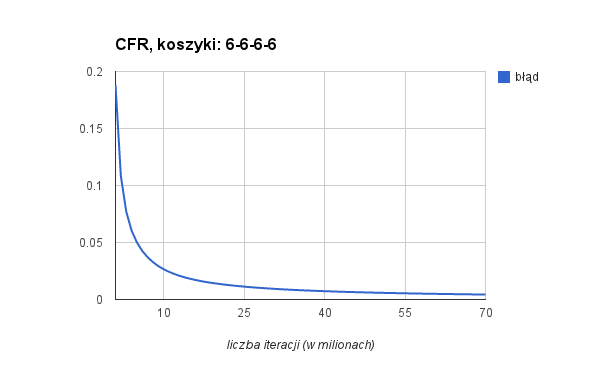
\includegraphics[scale=0.7]{wykres-cfr-6.png}

\noindent
Algorytm DAG CFR został policzony dla kilku zestawów koszyków: $(6,6,6,6)$, $(12,10,10,10)$ oraz $(19,19,19,19)$.
Jak widać, wymagał znacznie mniejszej liczby iteracji by zmniejszyć błąd do podobnego poziomu co w wywołaniu CFRa.

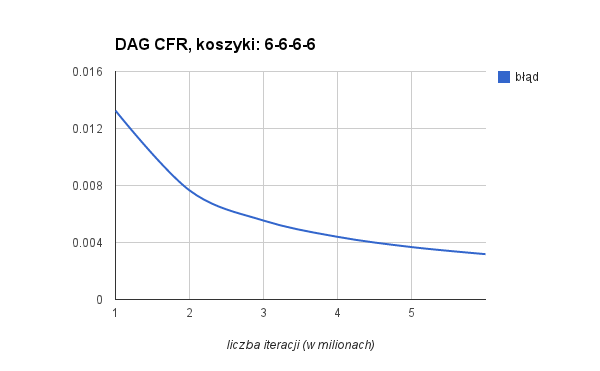
\includegraphics[scale=0.7]{wykres-dag-6.png}

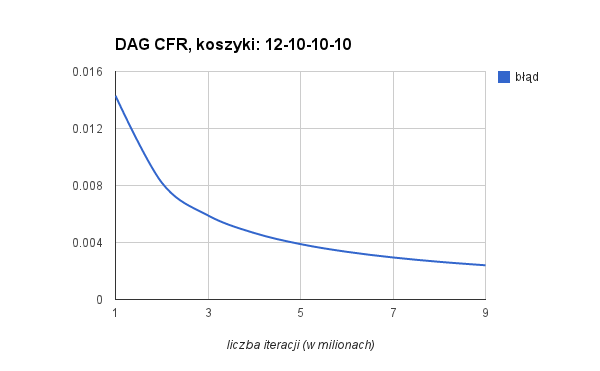
\includegraphics[scale=0.7]{wykres-dag-12.png}

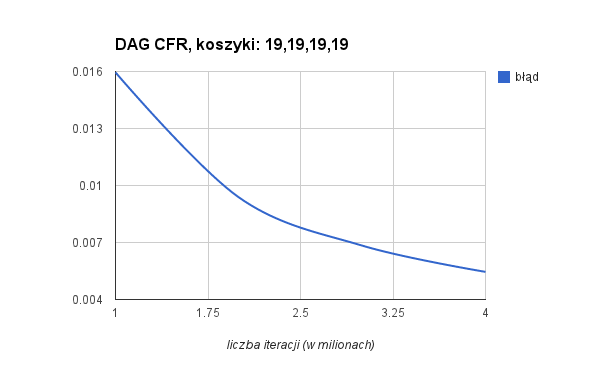
\includegraphics[scale=0.7]{wykres-dag-19.png}


$\,$ \\

\chapter{Podsumowanie}

\bibliographystyle{plain} 
\bibliography{cfr.bib} 

\end{document}
